% Options for packages loaded elsewhere
\PassOptionsToPackage{unicode}{hyperref}
\PassOptionsToPackage{hyphens}{url}
\PassOptionsToPackage{dvipsnames,svgnames,x11names}{xcolor}
%
\documentclass[
]{article}
\usepackage{amsmath,amssymb}
\usepackage{lmodern}
\usepackage{iftex}
\ifPDFTeX
  \usepackage[T1]{fontenc}
  \usepackage[utf8]{inputenc}
  \usepackage{textcomp} % provide euro and other symbols
\else % if luatex or xetex
  \usepackage{unicode-math}
  \defaultfontfeatures{Scale=MatchLowercase}
  \defaultfontfeatures[\rmfamily]{Ligatures=TeX,Scale=1}
\fi
% Use upquote if available, for straight quotes in verbatim environments
\IfFileExists{upquote.sty}{\usepackage{upquote}}{}
\IfFileExists{microtype.sty}{% use microtype if available
  \usepackage[]{microtype}
  \UseMicrotypeSet[protrusion]{basicmath} % disable protrusion for tt fonts
}{}
\makeatletter
\@ifundefined{KOMAClassName}{% if non-KOMA class
  \IfFileExists{parskip.sty}{%
    \usepackage{parskip}
  }{% else
    \setlength{\parindent}{0pt}
    \setlength{\parskip}{6pt plus 2pt minus 1pt}}
}{% if KOMA class
  \KOMAoptions{parskip=half}}
\makeatother
\usepackage{xcolor}
\usepackage[margin=1in]{geometry}
\usepackage{color}
\usepackage{fancyvrb}
\newcommand{\VerbBar}{|}
\newcommand{\VERB}{\Verb[commandchars=\\\{\}]}
\DefineVerbatimEnvironment{Highlighting}{Verbatim}{commandchars=\\\{\}}
% Add ',fontsize=\small' for more characters per line
\usepackage{framed}
\definecolor{shadecolor}{RGB}{248,248,248}
\newenvironment{Shaded}{\begin{snugshade}}{\end{snugshade}}
\newcommand{\AlertTok}[1]{\textcolor[rgb]{0.94,0.16,0.16}{#1}}
\newcommand{\AnnotationTok}[1]{\textcolor[rgb]{0.56,0.35,0.01}{\textbf{\textit{#1}}}}
\newcommand{\AttributeTok}[1]{\textcolor[rgb]{0.77,0.63,0.00}{#1}}
\newcommand{\BaseNTok}[1]{\textcolor[rgb]{0.00,0.00,0.81}{#1}}
\newcommand{\BuiltInTok}[1]{#1}
\newcommand{\CharTok}[1]{\textcolor[rgb]{0.31,0.60,0.02}{#1}}
\newcommand{\CommentTok}[1]{\textcolor[rgb]{0.56,0.35,0.01}{\textit{#1}}}
\newcommand{\CommentVarTok}[1]{\textcolor[rgb]{0.56,0.35,0.01}{\textbf{\textit{#1}}}}
\newcommand{\ConstantTok}[1]{\textcolor[rgb]{0.00,0.00,0.00}{#1}}
\newcommand{\ControlFlowTok}[1]{\textcolor[rgb]{0.13,0.29,0.53}{\textbf{#1}}}
\newcommand{\DataTypeTok}[1]{\textcolor[rgb]{0.13,0.29,0.53}{#1}}
\newcommand{\DecValTok}[1]{\textcolor[rgb]{0.00,0.00,0.81}{#1}}
\newcommand{\DocumentationTok}[1]{\textcolor[rgb]{0.56,0.35,0.01}{\textbf{\textit{#1}}}}
\newcommand{\ErrorTok}[1]{\textcolor[rgb]{0.64,0.00,0.00}{\textbf{#1}}}
\newcommand{\ExtensionTok}[1]{#1}
\newcommand{\FloatTok}[1]{\textcolor[rgb]{0.00,0.00,0.81}{#1}}
\newcommand{\FunctionTok}[1]{\textcolor[rgb]{0.00,0.00,0.00}{#1}}
\newcommand{\ImportTok}[1]{#1}
\newcommand{\InformationTok}[1]{\textcolor[rgb]{0.56,0.35,0.01}{\textbf{\textit{#1}}}}
\newcommand{\KeywordTok}[1]{\textcolor[rgb]{0.13,0.29,0.53}{\textbf{#1}}}
\newcommand{\NormalTok}[1]{#1}
\newcommand{\OperatorTok}[1]{\textcolor[rgb]{0.81,0.36,0.00}{\textbf{#1}}}
\newcommand{\OtherTok}[1]{\textcolor[rgb]{0.56,0.35,0.01}{#1}}
\newcommand{\PreprocessorTok}[1]{\textcolor[rgb]{0.56,0.35,0.01}{\textit{#1}}}
\newcommand{\RegionMarkerTok}[1]{#1}
\newcommand{\SpecialCharTok}[1]{\textcolor[rgb]{0.00,0.00,0.00}{#1}}
\newcommand{\SpecialStringTok}[1]{\textcolor[rgb]{0.31,0.60,0.02}{#1}}
\newcommand{\StringTok}[1]{\textcolor[rgb]{0.31,0.60,0.02}{#1}}
\newcommand{\VariableTok}[1]{\textcolor[rgb]{0.00,0.00,0.00}{#1}}
\newcommand{\VerbatimStringTok}[1]{\textcolor[rgb]{0.31,0.60,0.02}{#1}}
\newcommand{\WarningTok}[1]{\textcolor[rgb]{0.56,0.35,0.01}{\textbf{\textit{#1}}}}
\usepackage{graphicx}
\makeatletter
\def\maxwidth{\ifdim\Gin@nat@width>\linewidth\linewidth\else\Gin@nat@width\fi}
\def\maxheight{\ifdim\Gin@nat@height>\textheight\textheight\else\Gin@nat@height\fi}
\makeatother
% Scale images if necessary, so that they will not overflow the page
% margins by default, and it is still possible to overwrite the defaults
% using explicit options in \includegraphics[width, height, ...]{}
\setkeys{Gin}{width=\maxwidth,height=\maxheight,keepaspectratio}
% Set default figure placement to htbp
\makeatletter
\def\fps@figure{htbp}
\makeatother
\setlength{\emergencystretch}{3em} % prevent overfull lines
\providecommand{\tightlist}{%
  \setlength{\itemsep}{0pt}\setlength{\parskip}{0pt}}
\setcounter{secnumdepth}{-\maxdimen} % remove section numbering
\newlength{\cslhangindent}
\setlength{\cslhangindent}{1.5em}
\newlength{\csllabelwidth}
\setlength{\csllabelwidth}{3em}
\newlength{\cslentryspacingunit} % times entry-spacing
\setlength{\cslentryspacingunit}{\parskip}
\newenvironment{CSLReferences}[2] % #1 hanging-ident, #2 entry spacing
 {% don't indent paragraphs
  \setlength{\parindent}{0pt}
  % turn on hanging indent if param 1 is 1
  \ifodd #1
  \let\oldpar\par
  \def\par{\hangindent=\cslhangindent\oldpar}
  \fi
  % set entry spacing
  \setlength{\parskip}{#2\cslentryspacingunit}
 }%
 {}
\usepackage{calc}
\newcommand{\CSLBlock}[1]{#1\hfill\break}
\newcommand{\CSLLeftMargin}[1]{\parbox[t]{\csllabelwidth}{#1}}
\newcommand{\CSLRightInline}[1]{\parbox[t]{\linewidth - \csllabelwidth}{#1}\break}
\newcommand{\CSLIndent}[1]{\hspace{\cslhangindent}#1}
\ifLuaTeX
  \usepackage{selnolig}  % disable illegal ligatures
\fi
\IfFileExists{bookmark.sty}{\usepackage{bookmark}}{\usepackage{hyperref}}
\IfFileExists{xurl.sty}{\usepackage{xurl}}{} % add URL line breaks if available
\urlstyle{same} % disable monospaced font for URLs
\hypersetup{
  pdftitle={Searching spatial-temporal changes in intrinsic productivity of Antarctic Krill},
  pdfauthor={Mardones, M; Watters, G.; Cárdenas, C.},
  colorlinks=true,
  linkcolor={blue},
  filecolor={Maroon},
  citecolor={Blue},
  urlcolor={Blue},
  pdfcreator={LaTeX via pandoc}}

\title{Searching spatial-temporal changes in intrinsic productivity of
Antarctic Krill}
\usepackage{etoolbox}
\makeatletter
\providecommand{\subtitle}[1]{% add subtitle to \maketitle
  \apptocmd{\@title}{\par {\large #1 \par}}{}{}
}
\makeatother
\subtitle{Alternative analysis to know productivity in Krill 48.1
SubArea based on invariants parametres and fishery lenghts structures}
\author{Mardones, M; Watters, G.; Cárdenas, C.}
\date{18 May, 2023}

\begin{document}
\maketitle

\fontsize{12}{16}
\selectfont{}

\newpage

\setcounter{tocdepth}{3}
\tableofcontents

\newpage

\begin{Shaded}
\begin{Highlighting}[]
\FunctionTok{rm}\NormalTok{(}\AttributeTok{list =} \FunctionTok{ls}\NormalTok{())}
\NormalTok{knitr}\SpecialCharTok{::}\NormalTok{opts\_chunk}\SpecialCharTok{$}\FunctionTok{set}\NormalTok{(}\AttributeTok{echo =} \ConstantTok{FALSE}\NormalTok{,}
                      \AttributeTok{message =} \ConstantTok{FALSE}\NormalTok{,}
                      \AttributeTok{warning =} \ConstantTok{FALSE}\NormalTok{,}
                      \AttributeTok{fig.align =} \StringTok{\textquotesingle{}center\textquotesingle{}}\NormalTok{,}
                      \AttributeTok{dev =} \StringTok{\textquotesingle{}jpeg\textquotesingle{}}\NormalTok{,}
                      \AttributeTok{dpi =} \DecValTok{300}\NormalTok{,}
                      \AttributeTok{fig.width =} \DecValTok{6}\NormalTok{)}
\CommentTok{\#XQuartz is a mess, put this in your onload to default to cairo instead}
\FunctionTok{options}\NormalTok{(}\AttributeTok{bitmapType =} \StringTok{"cairo"}\NormalTok{) }
\CommentTok{\# (https://github.com/tidyverse/ggplot2/issues/2655)}
\CommentTok{\# Lo mapas se hacen mas rapido}
\end{Highlighting}
\end{Shaded}

\hypertarget{abstract}{%
\section{ABSTRACT}\label{abstract}}

Testing changes spatial and temporal in intrinsic productivity in
Antarctic Krill (\emph{Euphausia superba}) with Length-Based Spawning
Potential Ratio (LBSPR).

One way to understand krill dynamics is through empirical data such as
sizes structure from the fishery. In this sense we can, through the life
history parameters and the sizes through the years, what should be the
virgin reproductive potential (intrinsic productivity) and under the
effects of fishing.

Recognizing the intrinsic productivity changes of krill based on their
reproductive potential and how this changes in time and space, serves to
recognize the particularities of this species and the implications that
these results may have for management in the CCAMLR context.

\emph{Keywords: Lenght Structure, Intrinsic productivity, SPR, Krill,
48.1 SubArea}

\newpage

\hypertarget{introduction}{%
\section{1. INTRODUCTION}\label{introduction}}

The northern Antarctic Peninsula ecosystem is a critical region of the
Southern Ocean for populations of Antarctic krill (\emph{Euphausia
superba}; hereafter krill) serving as a major spawning and recruitment
area and as an overwintering hotspot, especially within Bransfield
Strait. Over the last 40 years, climate driven changes have resulted in
warming waters, declines in seasonal sea ice extent and duration
(\protect\hyperlink{ref-Stammerjohn2008a}{Sharon E. Stammerjohn et al.,
2008}; \protect\hyperlink{ref-Stammerjohn2008}{S. E. Stammerjohn et al.,
2008}), changing trends phytoplankton productivity
(\protect\hyperlink{ref-Saba2014}{Saba et al., 2014};
\protect\hyperlink{ref-Siegel2013}{Siegel et al., 2013}).

Additionally, changes have impacted the population dynamics of krill,
resulting in distribution changes with consequent contraction of the
population in the southwest Atlantic Ocean toward the peninsula
(\protect\hyperlink{ref-Atkinson2009}{A. Atkinson et al., 2009}). These
changes in the population structure have been verified in krill for the
last years also (\protect\hyperlink{ref-Reiss2020}{Reiss et al., 2020};
\protect\hyperlink{ref-Siegel2013}{Siegel et al., 2013}). This changes
(temporal and spatial) has implications for the reproductive potential
of the species and this, in turn, for intrinsic productivity.

One way to understand and measure changes in intrinsic productivity is
through assessing the ratio of krill reproductive potential. There are
many length-based assessment methods to understand this changes between
years (\protect\hyperlink{ref-Canales2021}{Canales et al., 2021};
\protect\hyperlink{ref-Froese2018}{Froese et al., 2018};
\protect\hyperlink{ref-Hordyk2016}{A. R. Hordyk et al., 2016};
\protect\hyperlink{ref-Rudd2017a}{Rudd \& Thorson, 2017}). On the other
hand, one of the advantages of these methods is to use one of the most
reliable and abundant sources in the sampling of fishing activities,
such as size structures (\protect\hyperlink{ref-Canales2021}{Canales et
al., 2021}).

This changes in spatial and temporal structure of krill population has
tried to be considered in management that performed CCAMLR (Commission
for the Conservation of Antarctic Marine Living Resources), but does not
consider reference points that can help in making decisions with
scientific rigor. We propose to identify the differences in the
reproductive potential of krill on the spatial and temporal scale,
propose a species-specific reference point and thereby provide
recommendations for the sustainable management of this fishery trough
Spawning Pontential Ratio (SPR) from krill population catch in SubArea
48.1 in Antarctic Peninsula in Southern Ocean.

\newpage

\hypertarget{methodology}{%
\section{2. METHODOLOGY}\label{methodology}}

\hypertarget{study-area}{%
\subsection{2.1. Study area}\label{study-area}}

The study area includes one of the sectors where today the largest
amount of krill fishing is concentrated. In this case, the analyzes
include the entire subarea 48.1. In order to have a better spatial
definition of the behavior of krill dynamics, we will analyze the
differences between the management strata defined in WG-EMM-2021/05
Rev.~(WG-EMM-2021/05 (\protect\hyperlink{ref-Dornam2021}{2021})), namely
Brainsfield Straith, Elephant Island, Extra, Joinville Island and South
West (Figure 1).

\begin{figure}
\centering
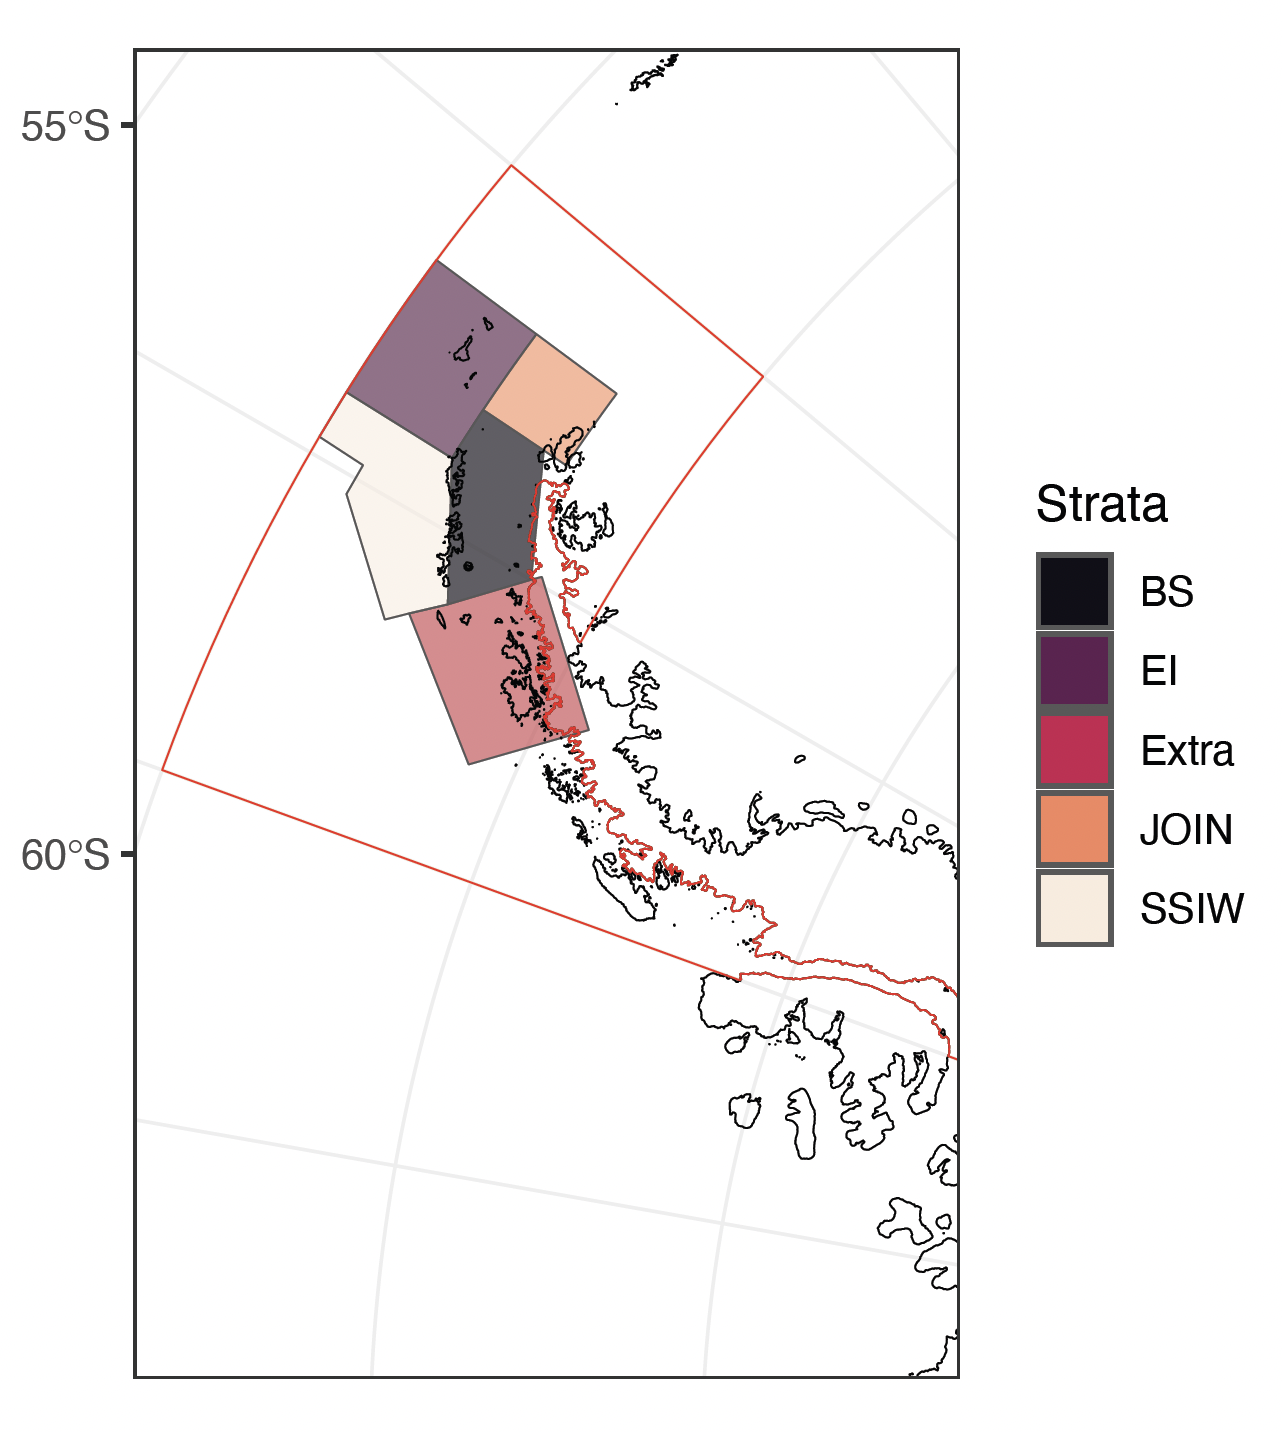
\includegraphics[width=0.6\textwidth,height=\textheight]{Strata2.png}
\caption{Figure 1. Subarea 48.1 and management strata considered in the
spatio-temporal analysis of intrinsic productivity of Krill
(BS=Brainsfield Straith, EI= Elephant Island, Extra= Extra, JOIN=
Joinville Island, SSWI= South West) West)}
\end{figure}

\hypertarget{data}{%
\subsection{2.2. Data}\label{data}}

For this analysis, data from the monitoring of the krill fishery were
used, which have been systematically collected on board fishing vessels
by the SISO (Scheme of International Scientific Observation) program
carried out by CCAMLR. Krill sizes compositions were obtained from the
entire area 48.1, which was joined in each management stratum defined at
2.1 section.

\hypertarget{assessment-of-intrinsic-productivity}{%
\subsection{2.3 Assessment of intrinsic
productivity}\label{assessment-of-intrinsic-productivity}}

The intrinsic productivity of krill was evaluated through a method that
measures the reproductive potential of commercially exploited marine
species known as LB-SPR (Length Based Spawining Potential Ratio) and
described by A. R. Hordyk et al.
(\protect\hyperlink{ref-Hordyk2016}{2016}). The LB-SPR method has been
developed for data-limited fisheries, where few data are available other
than a representative sample of the size structure of the vulnerable
portion of the population (i.e., the catch) and an understanding of the
life history of the species. The LBSPR method assumes the reproductive
characteristics of the species based on the life history parameters,
being able to establish strategies for long-lived species with low
reproductive output as well as highly reproductive species with a high
growth constant such as krill (\protect\hyperlink{ref-Prince2018}{Prince
\& Hordyk, 2018}).

LBSPR uses length-composition data and assumptions about biological
parameters to make a rapid assessment of stock status relative to
unfished levels assuming equilibrium conditions. While LB-SPR can use
multiple years of length data, status determination is based on one year
of data at a time (i.e., estimates of status over multiple years are
based on that year's length composition alone). Mean-length mortality
estimators, first developed by Beverton \& Holt
(\protect\hyperlink{ref-Beverton1957}{1957}), assume that fishing
mortality directly influences mean length of the catch and therefore in
the reproductive potential of the species. Al l this concept about life
history and implications in spawning potential ratio was revisited by
Jensen (\protect\hyperlink{ref-Jensen1996}{1996}).

here are two versions of the LB-SPR model included in this methodology.

\hypertarget{life-story-and-fishery-parameters}{%
\subsection{2.5. Life story and fishery
parameters}\label{life-story-and-fishery-parameters}}

\begin{verbatim}
##  [1] "Species"      "MK"           "M"            "Linf"         "L_units"     
##  [6] "CVLinf"       "L50"          "L95"          "Walpha"       "Walpha_units"
## [11] "Wbeta"        "FecB"         "Steepness"    "Mpow"         "R0"          
## [16] "SL50"         "SL95"         "MLL"          "sdLegal"      "fDisc"       
## [21] "FM"           "SPR"          "BinMin"       "BinMax"       "BinWidth"
\end{verbatim}

The model needs specifications related to both biological and fishery
parameters according to the taxonomic group evaluated. These
specifications are compiled in technical reports and/or indexed
publications about krill life history and fishery
(\protect\hyperlink{ref-Maschette2020}{Maschette et al., 2020};
\protect\hyperlink{ref-Thanassekos2014}{Thanassekos et al., 2014}),
which are described in Table 1.

In a descriptive way, the main parameter sets are described as follows;

\textbf{Biology}

\begin{itemize}
\tightlist
\item
  von Bertalanffy asymptotic length \texttt{Linf}
\item
  M/K ratio (natural mortality)divided by von Bertalanffy K coefficient)
  \texttt{MK}
\item
  Length at 50\% maturity (\texttt{L50})
\item
  Length at 95\% maturity (\texttt{L95})
\end{itemize}

\textbf{Fishery}

\begin{itemize}
\tightlist
\item
  Length at 50\% selectivity (\texttt{SL50})
\item
  Length at 95\% selectivity (\texttt{SL95})
\item
  Biological Reference Point (BRP). F/M ratio (\texttt{FM}) or Spawning
  Potential Ratio (\texttt{SPR}). If you specify both, the F/M value
  will be ignored.
\end{itemize}

Size Classes

-Width of the length classes (\texttt{BinWidth})

\hypertarget{model-estimation-lb-spr}{%
\subsection{2.4. Model Estimation
LB-SPR}\label{model-estimation-lb-spr}}

Recent work has shown that, under equilibrium conditions (that is,
constant F and no recruitment variability) and assuming the von
Bertalanffy growth equation, constant natural mortality for all ages,
and logistic or jack-knife selectivity, standardization of the
composition of lengths of two populations with the same ratio of natural
mortality to growth rate (M/k) and the same ratio of mortality by
fishing to natural mortality (F/M) will be identical
(\protect\hyperlink{ref-Hordyk2016}{A. R. Hordyk et al., 2016}).
Extension of this model to incorporate length-at-age variability and
logistic selectivity confirms that, at equilibrium, the composition of
the predicted duration of catch of an exploited population is primarily
determined by the ratios of M/k and F/M. The analytical models developed
in A. Hordyk et al. (\protect\hyperlink{ref-Hordyk2014c}{2014}) suggest
that with knowledge of the asymptotic von Bertalanffy length
L\_\{\infty\} and the coefficient of variation in CVL\_\{\infty\}, the
ratio of total mortality to the von Bertalanffy growth coefficient (Z
/k) for a given population can be estimated from a representative sample
of the size structure of the catch. If M/k is also known (from
meta-analyses, life history theory, expert opinion, or population
biological studies), then the results of A. R. Hordyk et al.
(\protect\hyperlink{ref-Hordyk2016}{2016}) suggest that it is possible
to estimate F/M from the composition of the catch. Often the F/M ratio
has been used as a biological reference point when is 1
(\protect\hyperlink{ref-Zhou2012}{Zhou et al., 2012}).

The LB-SPR model requires the following parameters: an estimate of the
M/k ratio, L\_inf, CVL\_inf, and knowledge of maturity by length
(maturity ogive), both know in krill. This model uses data on
composition by catch sizes to estimate intrinsic productivity or SPR.
This concept was calculated following Goodyear
(\protect\hyperlink{ref-Goodyear1993}{1993}), where he calculated the
ratio between the average lifetime egg production per recruit (EPR) in
equilibrium for fish and non-fish resources, assuming density-dependent
suppression of maturity or fecundity.

\[{SPR}=\frac{EPR_{fished}}{EPR_{nofished}}\] where;

\[
EPR_{fished} =
\sum_{a}
\begin{cases}
 EPR_{a},  a = 0  \\
 e^{-Z_{{a-1}}a EPR_a}, 0 < a  < a_{max}
 \end{cases}       
\] where \(Z_a\) = M + \(S_a\)*F, and;

\[
EPR_{nofished} =
\sum_{a}
 EPR_ae^{-Mas}
\] Assuming that egg production is proportional to the size of mature
fish, relative fecundity-at-size is given by;

\[
Fec_{L,g} = Mat_{L,g} L^b
\] where b is value of the exponent to reflect differente size
fecunditity relationship and g is the fraction of recruits to group.

Assuming reasonable estimates of the M/K ratio, \(L_{\infty}\) (or
\(CVL_{\infty}\)), size-at-maturity, the parameters F/M, \(SL_{50}\),
and \(SL_{95}\) can be estimated from a representative sample of the
length structure of the catch by minimizing the following multinomial
negative loglikelihood function (NLL):

\[
NLL =
argmin\sum_{i}
 O_i ln\frac{\hat{P}_i}{\hat{O}_i}
\]

where \(O_i\) and \(\hat{O}_i\) are the observed number and proportion
in length class i, respectively, and \(\hat{P}_i\) is the model estimate
of the probability in length class i
(\protect\hyperlink{ref-Hordyk2016}{A. R. Hordyk et al., 2016}).

The LBSPR model described by (\protect\hyperlink{ref-Hordyk2014c}{A.
Hordyk et al., 2014}; \protect\hyperlink{ref-Hordyk2016}{A. R. Hordyk et
al., 2016}), and tested in a MSE framework
(\protect\hyperlink{ref-Hordyk2014c}{A. Hordyk et al., 2014}), use a
conventional age-structured equilibrium population model. An important
assumption of this model structure is that selectivity is age-based not
length-based. A. R. Hordyk et al.
(\protect\hyperlink{ref-Hordyk2016}{2016}) describe a length-structured
version of the LBSPR model that uses growth-type-groups (GTG) to account
for size-based selectivity. The GTG-LBSPR model also has the ability to
include variable M at size (by default M is assumed to be constant). The
GTG-LBSPR model typically estimates a lower fishing mortality rate for a
given size structure compared to the earlier age-structured model. This
is because the age-structured model has a `regeneration assumption',
where, because of the age-based selectivity assumption, large
individuals are expected even at high fishing mortality (large, young
fish).

The default setting for the LBSPR package is to use the GTG-LBSPR model
for all simulation and estimation. Control options in the simulation and
estimation functions can be used to switch to the age-structured LBSPR
model.

Like any assessment method, the LBSPR model relies on a number of
simplifying assumptions. In particular, the LBSPR models are equilibrium
based, and assume that the length composition data is representative of
the exploited population at steady state. This methodology was
implemented through the package A. Hordyk
(\protect\hyperlink{ref-LBSPR2021}{2021}).

\hypertarget{references-point-in-krill-fishery}{%
\subsection{2.4. References Point in Krill
fishery}\label{references-point-in-krill-fishery}}

A constant challenge for length-based methods has been to provide
indicators of stock status that can be compared to predetermined
biological reference points. The spawning potential ratio (SPR) of a
stock is defined as the proportion of potential unexploited spawning at
any given level of fishing pressure (Goodyear, 1993; Walters and
Martell, 2004) and is commonly used to set the target points. limit and
target reference. By definition, the SPR is equal to 100\% in an
unexploited stock, and zero in a non-spawning stock (eg all mature fish
have been removed, or all females have been caught). The F40\%, that is,
the fishing mortality rate that translates into SPR = 40\%, is
considered risky for many species (Clark, 2002). Suitable SPR biological
points can be derived from hypotheses about the steepness of the
stock-recruit relationship (Brooks et al., 2010). Hordyk et al.~(2015)
show that, under the assumptions of razor-edge selectivity for length at
Lc, and maturity at Lm, the SPR is determined by the ratios of M / k, F
/ M, Lm / L\^{}, and Lc /L\^{}.

As measures of stock status, these length-based methods derive the
spawning potential ratio (SPR) reference point, defined as the
proportion of unfished reproductive potential at a given level of
fishing pressure (\protect\hyperlink{ref-Goodyear1993}{Goodyear, 1993}).

There are three management rules for krill (Constable et al 2000):

\begin{enumerate}
\def\labelenumi{(\arabic{enumi})}
\item
  the median krill spawning biomass over a 20-year period should not
  fall below 75\% of its pre-exploitation median level (PBR Obj ó MSY
  (Hill et al., 2016);
\item
  the probability that krill spawning biomass drops below 20\% of its
  pre-exploitation median level over a 20-year harvesting period should
  not exceed 10\%; (PBR Limit)
\end{enumerate}

\newpage

\hypertarget{simulation}{%
\subsection{2.4. Simulation}\label{simulation}}

The LBSPR package can be used to generate the expected size composition,
the SPR, and relative yield for a given set of biological and
exploitation pattern parameters.

\hypertarget{lb_pars-object-to-antarctic-krill}{%
\subsection{2.5. LB\_pars Object to Antarctic
Krill}\label{lb_pars-object-to-antarctic-krill}}

The first thing to do is to create a LB\_pars object that contains all
of the required parameters for the simulation model. LB\_pars is an S4
class object.

\hypertarget{populate-the-lb_pars-object-with-krill-parameters}{%
\paragraph{2.5.2. Populate the LB\_pars Object with Krill
parameters}\label{populate-the-lb_pars-object-with-krill-parameters}}

\hypertarget{running-the-simulation-model}{%
\subsection{2.6. Running the Simulation
Model}\label{running-the-simulation-model}}

Now we are ready to run the LBSPR simulation model. To do this we use
the LBSPRsim function: ngtg function es el \# de grupos para el GTG
model, por default es 13)

\begin{Shaded}
\begin{Highlighting}[]
\NormalTok{MySim }\OtherTok{\textless{}{-}} \FunctionTok{LBSPRsim}\NormalTok{(MyPars, }
                  \AttributeTok{Control=}\FunctionTok{list}\NormalTok{(}\AttributeTok{modtype=}\StringTok{"GTG"}\NormalTok{, }
                               \AttributeTok{maxFM=}\DecValTok{1}\NormalTok{)) }
\end{Highlighting}
\end{Shaded}

\hypertarget{the-lb_obj-object}{%
\paragraph{2.6.1. The LB\_obj Object}\label{the-lb_obj-object}}

The output of the LBSPRsim function is an object of class LB\_obj. This
is another S4 object, and contains all of the information from the
LB\_pars object and the output of the LBSPRsim function.

Many of the functions in the LBSPR package return an object of class
LB\_obj. You should not modify the LB\_obj object directly. Rather, make
changes to the LB\_pars object (MyPars in this case), and re-run the
simulation model (or other functions, covered later in the vignette).

\hypertarget{simulation-output}{%
\paragraph{2.6.2. Simulation Output}\label{simulation-output}}

Let's take a look at some of the simulated output.

\begin{Shaded}
\begin{Highlighting}[]
\NormalTok{MySim}\SpecialCharTok{@}\NormalTok{SPR }
\end{Highlighting}
\end{Shaded}

\begin{verbatim}
## [1] 0.75
\end{verbatim}

The simulated SPR is the same as our input value \texttt{MyPars@SPR}

What is the ratio of fishing mortality to natural mortality in this
scenario?

\begin{verbatim}
## [1] 0.29
\end{verbatim}

It is important to note that the F/M ratio reported in the LBSPR model
refers to the apical F over the adult natural mortality rate. That is,
the value for fishing mortality refers to the highest level of F
experienced by any single size class.

If the selectivity pattern excludes all but the largest individuals from
being exploited, it is possible to have a very high F/M ratio in a
sustainable fishery (high SPR). And visceverse!!

\hypertarget{control-options}{%
\paragraph{2.6.3. Control Options}\label{control-options}}

There are a number of additional parameters that can be modified to
control other aspects of the simulation model.

For example, by default the LBSPR model using the Growth-Type-Group
model (Hordyk et at. 2016). The Control argument can be used to switch
to the Age-Structured model (Hordyk et al.~2015a, b):

See the help file for the LBSPRsim function for additional parameters
for the Control argument.

\hypertarget{plotting-the-simulation}{%
\paragraph{2.6.4. Plotting the
Simulation}\label{plotting-the-simulation}}

The plotSim function can be used to plot MySim:

\begin{figure}

{\centering \includegraphics{indexPDF_files/figure-latex/unnamed-chunk-7-1} 

}

\caption{Ploteo de Simulaci?n estructuras.}\label{fig:unnamed-chunk-7}
\end{figure}

By default the function plots: a) the expected (equilibrium) size
structure of the catch and the expected unfished size structure of the
vulnerable population, b) the maturity and selectivity-at-length curves,
c) the von Bertalanffy growth curve with relative age, and d) the SPR
and relative yield curves as a function of relative fishing mortality
(see note above on the F/M ratio).

The plotSim function can be controlled in a number of ways. For example,
you can plot the expected unfished and fished size structure of the
population by changing the lf.type argument:

\begin{figure}

{\centering \includegraphics{indexPDF_files/figure-latex/unnamed-chunk-8-1} 

}

\caption{Ploteo de Simulaci?n Population.}\label{fig:unnamed-chunk-8}
\end{figure}

Individual plots can be created using the type argument:

\begin{figure}

{\centering \includegraphics{indexPDF_files/figure-latex/unnamed-chunk-9-1} 

}

\caption{Plot Leng Freq}\label{fig:unnamed-chunk-9}
\end{figure}

See ?plotSim for more options for plotting the output of the LBSPR
simulation model.

\newpage

\hypertarget{fitting-empirical-krill-length-data}{%
\subsection{2.7 Fitting Empirical Krill Length
Data}\label{fitting-empirical-krill-length-data}}

Two objects are required to fit the LBSPR model to length data: LB\_pars
which contains the life-history parameters (described above) and
LB\_lengths, which contains the length frequency data.

\hypertarget{creating-a-lb_lengths-object}{%
\paragraph{2.7.1 Creating a LB\_lengths
object}\label{creating-a-lb_lengths-object}}

A LB\_lengths object can be created in two ways. The new function can be
used to create an empty object which can be manually populated:

\begin{Shaded}
\begin{Highlighting}[]
\FunctionTok{slotNames}\NormalTok{(MyLengths)}
\end{Highlighting}
\end{Shaded}

\begin{verbatim}
## [1] "LMids"   "LData"   "L_units" "Years"   "NYears"  "Elog"
\end{verbatim}

However, it is probably easier to create the LB\_lengths object by
directly reading in a \texttt{CSV\ file}.

Now, we need set our directory again

\hypertarget{reading-krill-data}{%
\paragraph{2.7.2 Reading Krill Data}\label{reading-krill-data}}

Note that only the life history parameters need to be specified for the
estimation model. The exploitation parameters will be estimated.

A length frequency data of krill set with multiple years (2001-2020):

\begin{Shaded}
\begin{Highlighting}[]
\NormalTok{Len1 }\OtherTok{\textless{}{-}} \FunctionTok{new}\NormalTok{(}\StringTok{"LB\_lengths"}\NormalTok{, }\AttributeTok{LB\_pars=}\NormalTok{MyPars, }\AttributeTok{file=}\FunctionTok{paste0}\NormalTok{(datdir, }\StringTok{"/Length\_481\_Krill\_2.csv"}\NormalTok{), }\AttributeTok{dataType=}\StringTok{"freq"}\NormalTok{,}\AttributeTok{sep=}\StringTok{";"}\NormalTok{,}\AttributeTok{header=}\NormalTok{T)}
\end{Highlighting}
\end{Shaded}

Another form to read data is: A length frequency data set with multiple
years and a header row (identical to Len1 data, but with a header row):

\hypertarget{plotting-length-data-krill}{%
\paragraph{2.7.3 Plotting Length Data
Krill}\label{plotting-length-data-krill}}

The \texttt{plotSize} function can be used to plot the imported length
data. This is usually a good idea to do before proceeding with fitting
the model, to confirm that everything has been read in correctly:

\begin{center}\includegraphics{indexPDF_files/figure-latex/unnamed-chunk-14-1} \end{center}

\hypertarget{fit-the-model}{%
\subsubsection{2.7.4. Fit the Model}\label{fit-the-model}}

The LBSPR model is fitted using the \texttt{LBSPRfit} function:

Note that the Control argument can be used to modify the additional
parameters or LBSPR model type (see description in earlier section).

\hypertarget{results}{%
\section{3. RESULTS}\label{results}}

This consideration is because we have different size structure in each
strata, like we can see in this figure.

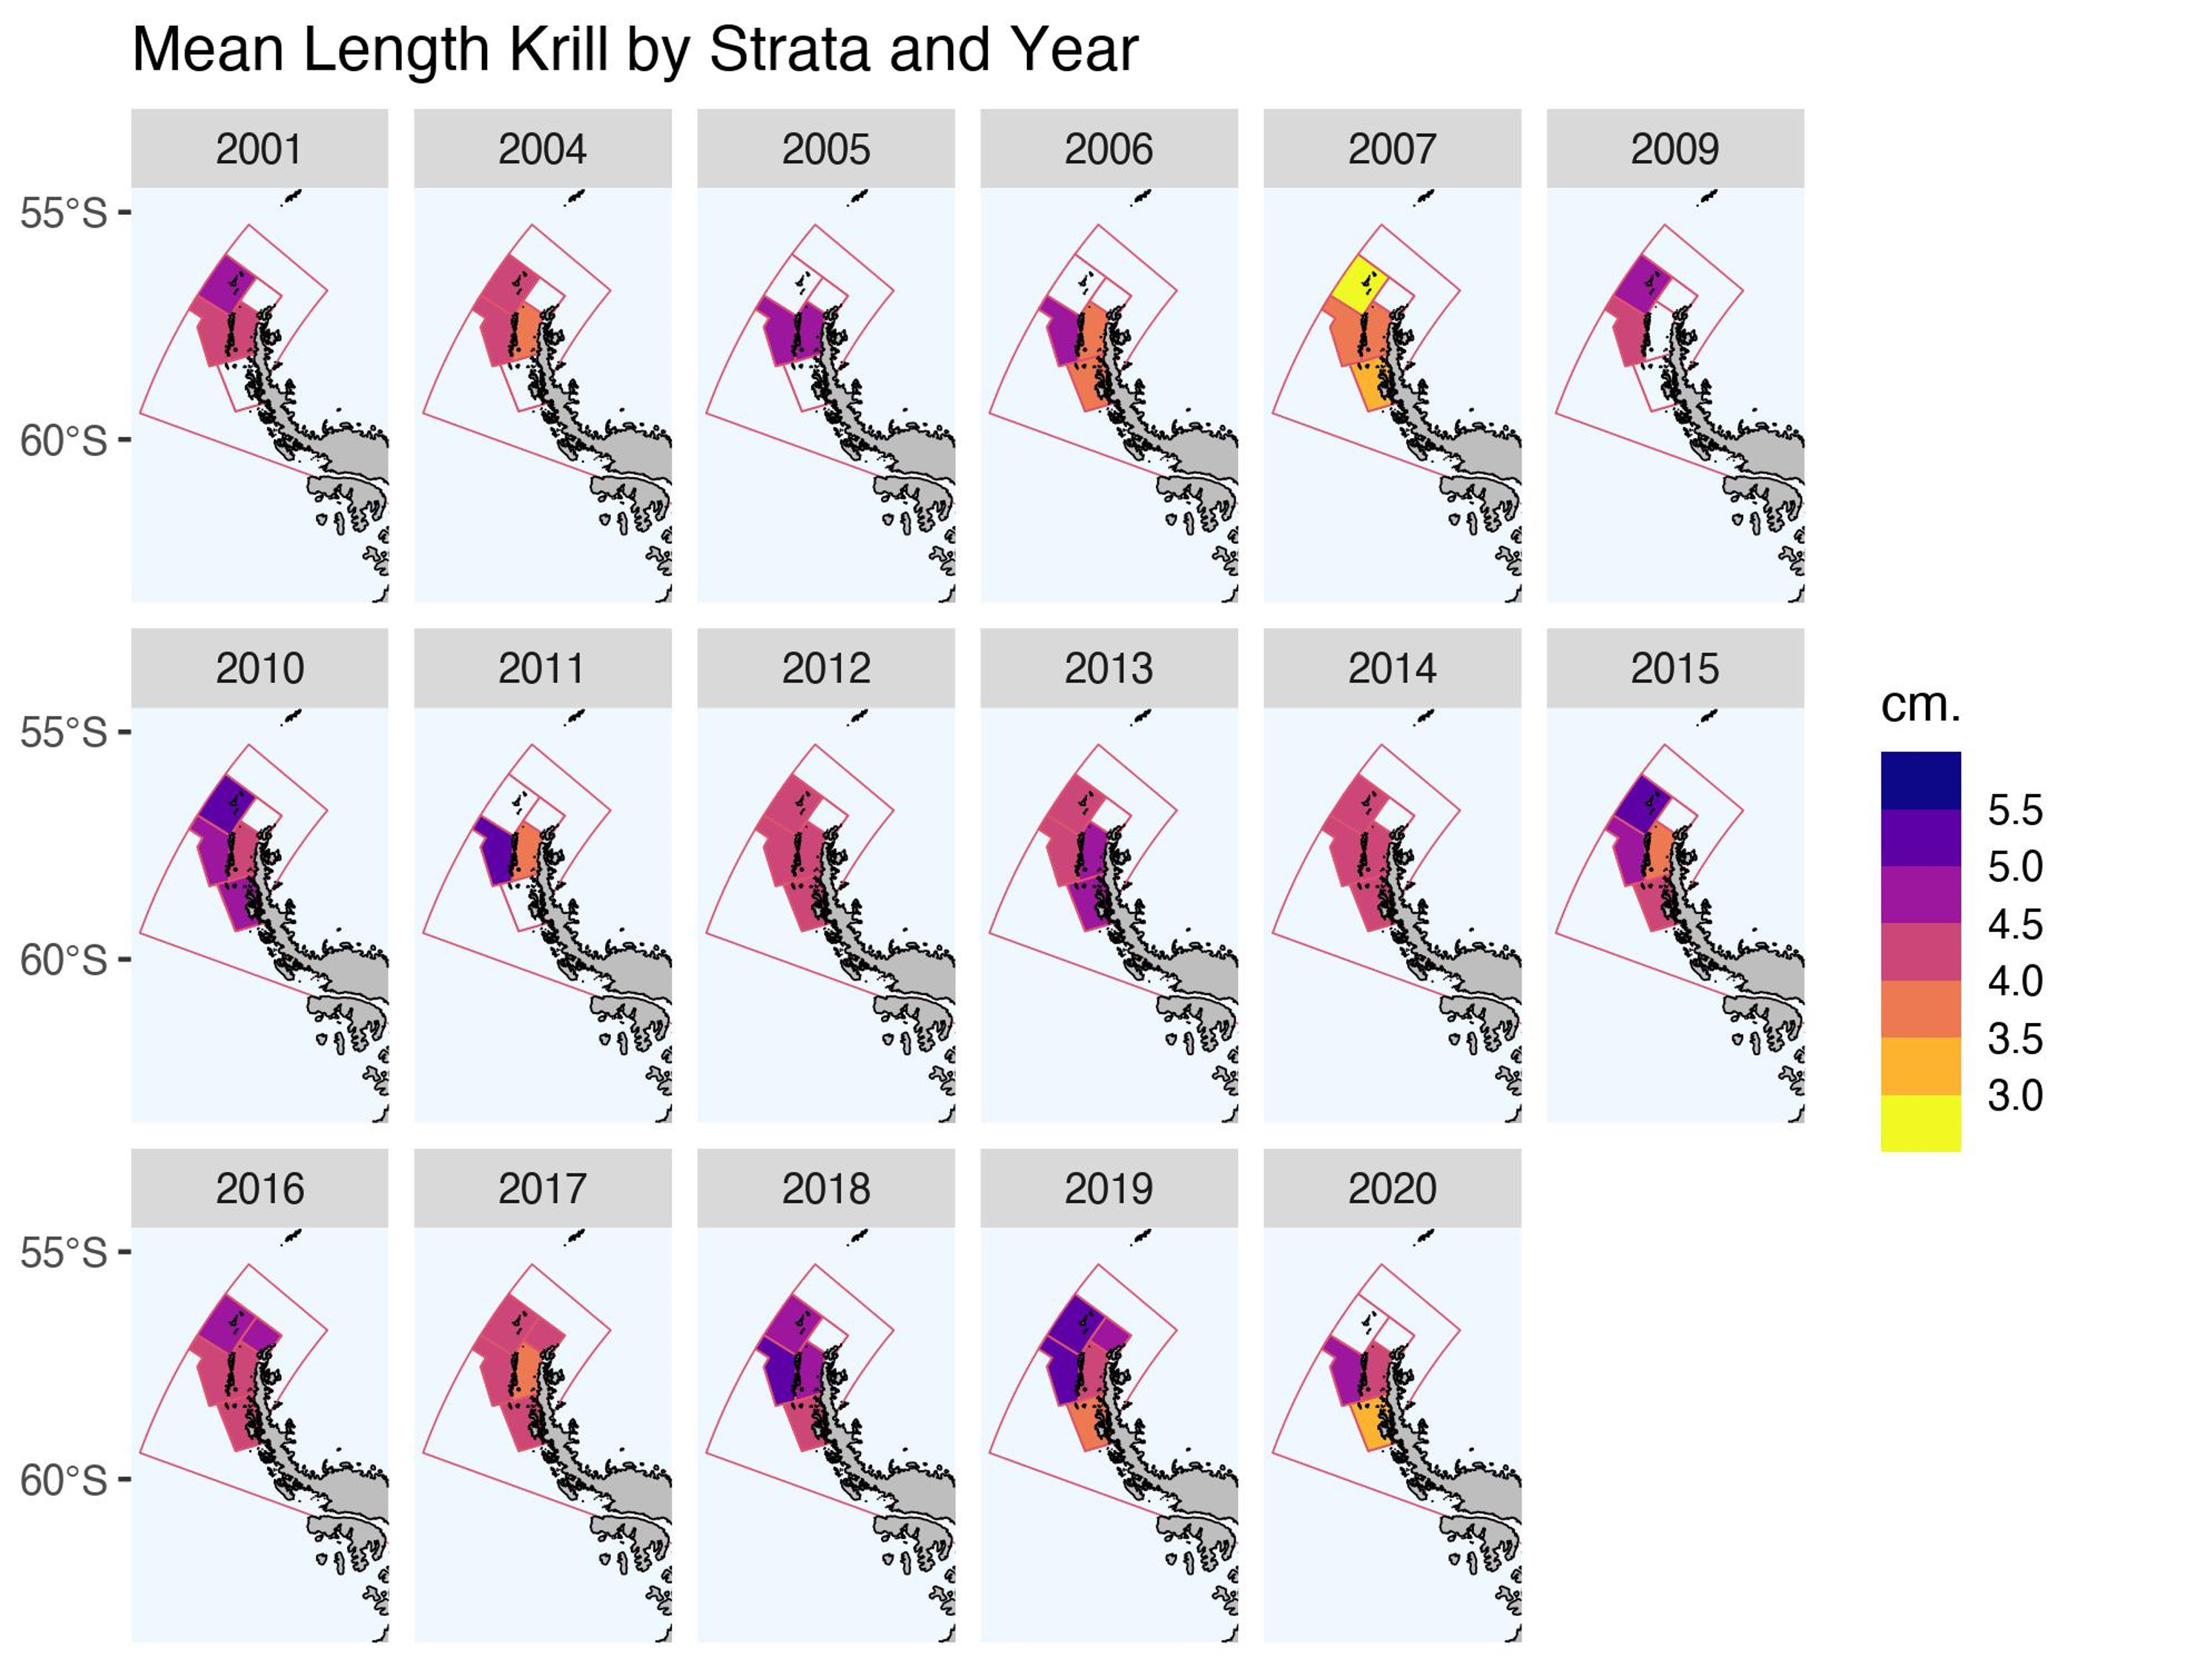
\includegraphics{StrataLen.jpg} With this differences, we proceed to
search intrinsic productivity (Spawning Potential Ratio) by strata and
by years.

The LBSPR package uses a Kalman filter and the Rauch-Tung-Striebel
smoother function (see FilterSmooth) to smooth out the multi-year
estimates of SPR, F/M, and selectivity parameters.

The smoother parameter estimates can be accessed from the \texttt{myFit}
object (which is an object of class LB\_obj {[}see earlier section for
details{]}):

\begin{Shaded}
\begin{Highlighting}[]
\NormalTok{myFit1}\SpecialCharTok{@}\NormalTok{Ests}
\end{Highlighting}
\end{Shaded}

\begin{verbatim}
##        SL50  SL95   FM  SPR
##  [1,] 45.59 55.77 5.35 0.30
##  [2,] 44.96 54.87 5.02 0.29
##  [3,] 44.87 54.76 4.80 0.30
##  [4,] 44.77 55.29 4.55 0.30
##  [5,] 44.28 55.03 4.27 0.30
##  [6,] 43.40 53.99 4.08 0.29
##  [7,] 43.78 54.25 4.00 0.30
##  [8,] 44.15 54.74 3.91 0.32
##  [9,] 44.33 55.09 3.78 0.33
## [10,] 43.29 54.10 3.60 0.31
## [11,] 42.32 52.54 3.61 0.29
## [12,] 42.11 52.25 3.72 0.28
## [13,] 41.98 52.36 3.77 0.27
## [14,] 41.69 52.32 3.72 0.27
## [15,] 40.93 51.55 3.68 0.26
## [16,] 40.22 50.59 3.64 0.25
## [17,] 39.48 49.77 3.56 0.25
## [18,] 39.13 49.35 3.68 0.24
\end{verbatim}

Note that by default the smoothed estimates are used in the plotting
routines.

The individual point estimates for each year can be accessed from the
\texttt{LB\_obj} object:

\begin{Shaded}
\begin{Highlighting}[]
\FunctionTok{data.frame}\NormalTok{(}\AttributeTok{rawSL50=}\NormalTok{myFit1}\SpecialCharTok{@}\NormalTok{SL50, }\AttributeTok{rawSL95=}\NormalTok{myFit1}\SpecialCharTok{@}\NormalTok{SL95, }\AttributeTok{rawFM=}\NormalTok{myFit1}\SpecialCharTok{@}\NormalTok{FM, }\AttributeTok{rawSPR=}\NormalTok{myFit1}\SpecialCharTok{@}\NormalTok{SPR)}
\end{Highlighting}
\end{Shaded}

\begin{verbatim}
##    rawSL50 rawSL95 rawFM    rawSPR
## 1    52.44   65.34  8.69 0.3390804
## 2    39.43   46.97  3.92 0.2087088
## 3    45.01   48.33  5.11 0.3251658
## 4    48.63   63.15  4.89 0.3141996
## 5    48.24   62.96  3.30 0.3718446
## 6    30.72   40.89  3.04 0.1254271
## 7    44.01   51.94  4.00 0.2960077
## 8    45.92   56.19  4.39 0.3095126
## 9    56.55   68.49  4.31 0.5789779
## 10   42.64   59.75  1.64 0.3952354
## 11   34.69   39.89  2.65 0.1931645
## 12   41.36   48.17  4.35 0.2346415
## 13   43.51   53.96  4.71 0.2468353
## 14   46.46   59.59  3.59 0.3306032
## 15   40.44   53.47  3.74 0.2114859
## 16   40.45   49.14  4.10 0.2164218
## 17   35.63   45.84  1.40 0.3311026
## 18   35.62   45.10  4.97 0.1211154
\end{verbatim}

The \texttt{plotSize} function can also be used to show the model fit to
the data:

\begin{center}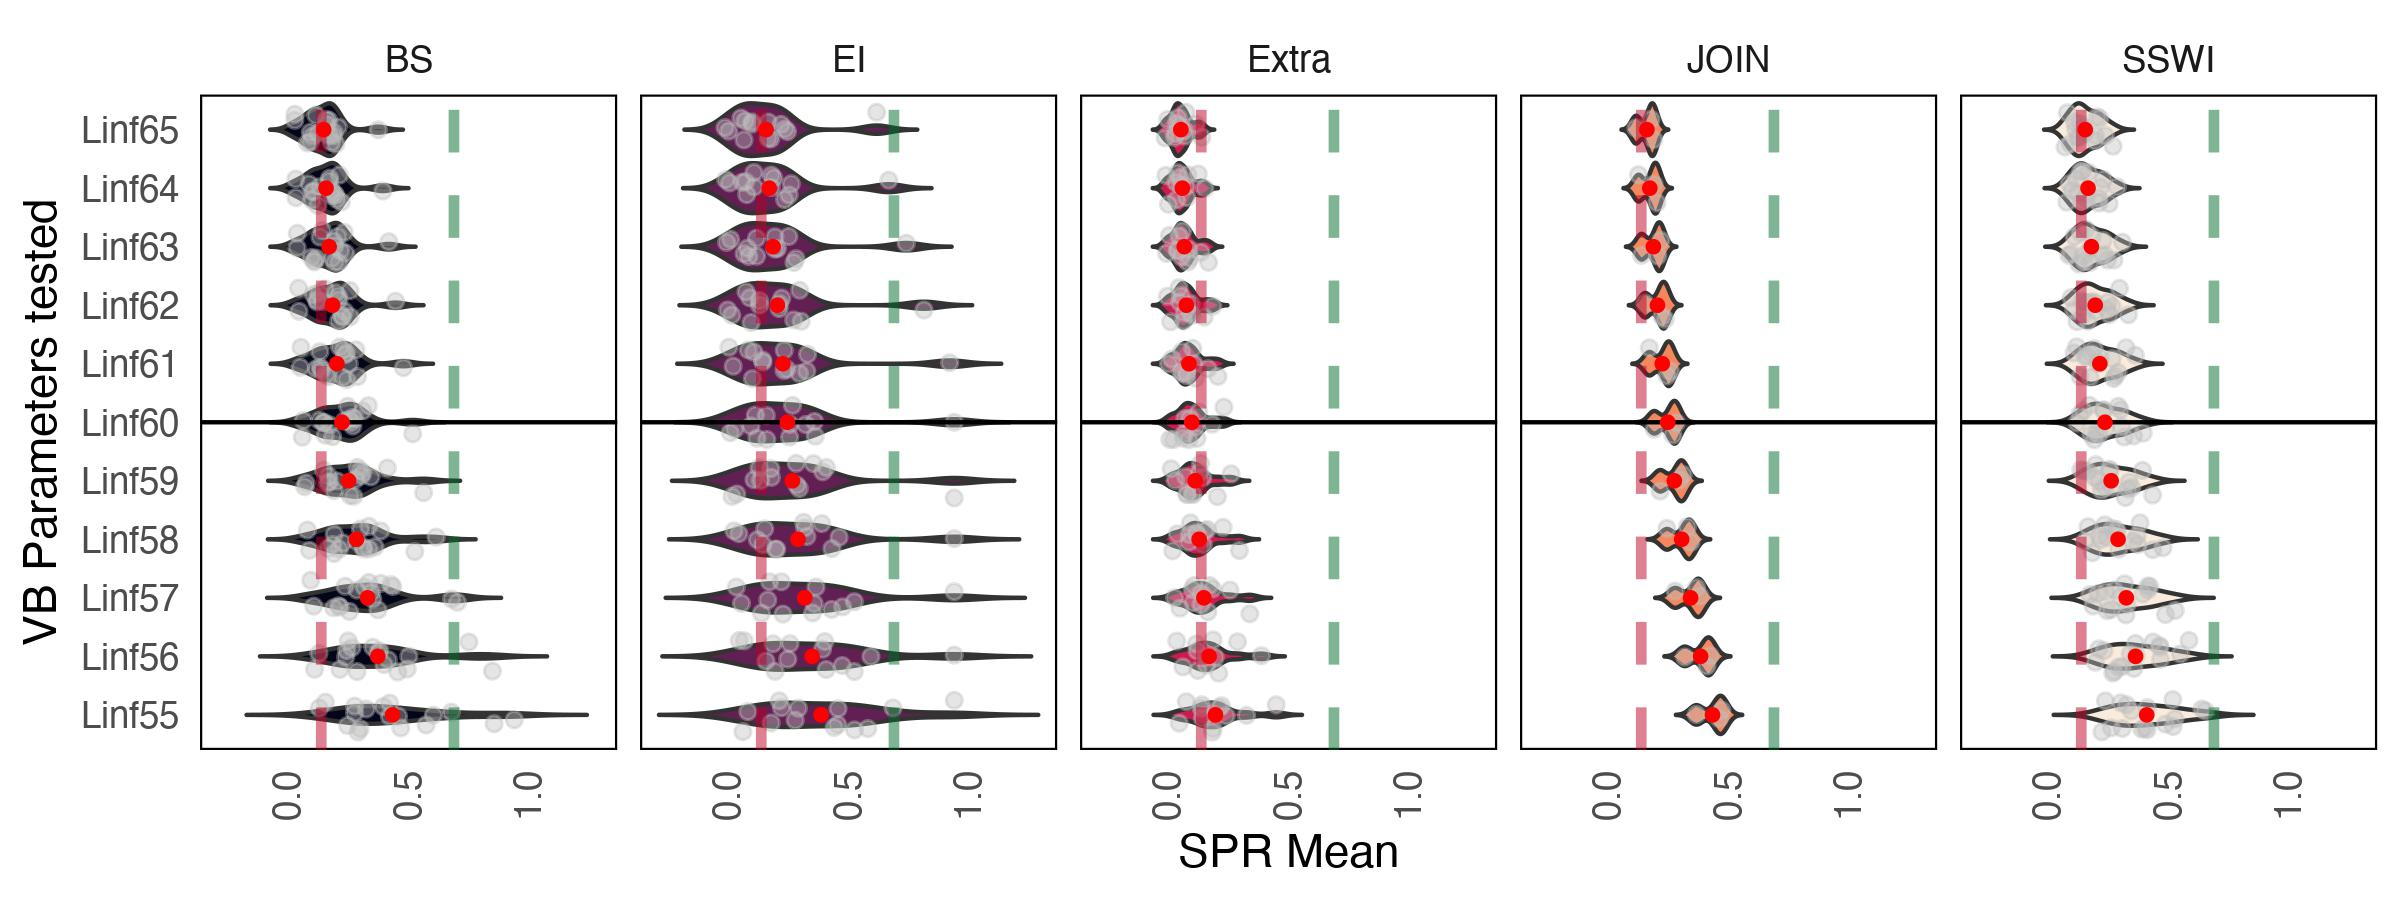
\includegraphics{indexPDF_files/figure-latex/unnamed-chunk-18-1} \end{center}

Similarly, the plotMat function can be used to show the specified
maturity-at-length curve, and the estimated selectivity-at-length curve:

\begin{center}\includegraphics{indexPDF_files/figure-latex/unnamed-chunk-19-1} \end{center}

Finally, the plotEsts function can be used to visually display the
estimated parameters. Note that this works for all data sets, but only
makes sense when there are several years of data:

\begin{center}\includegraphics{indexPDF_files/figure-latex/unnamed-chunk-20-1} \end{center}

By default the plotting function adds the smoother line to the estimated
points.

\newpage

\hypertarget{comparing-observed-length-data-to-target-size-structure}{%
\subsection{3.1. Comparing Observed Length Data to Target Size
Structure}\label{comparing-observed-length-data-to-target-size-structure}}

You can compare the observed size data against an expected size
composition at a target SPR using the \texttt{plotTarg} function. To do
this, you need a LB\_pars object with the life history parameters and
the target SPR:

\begin{center}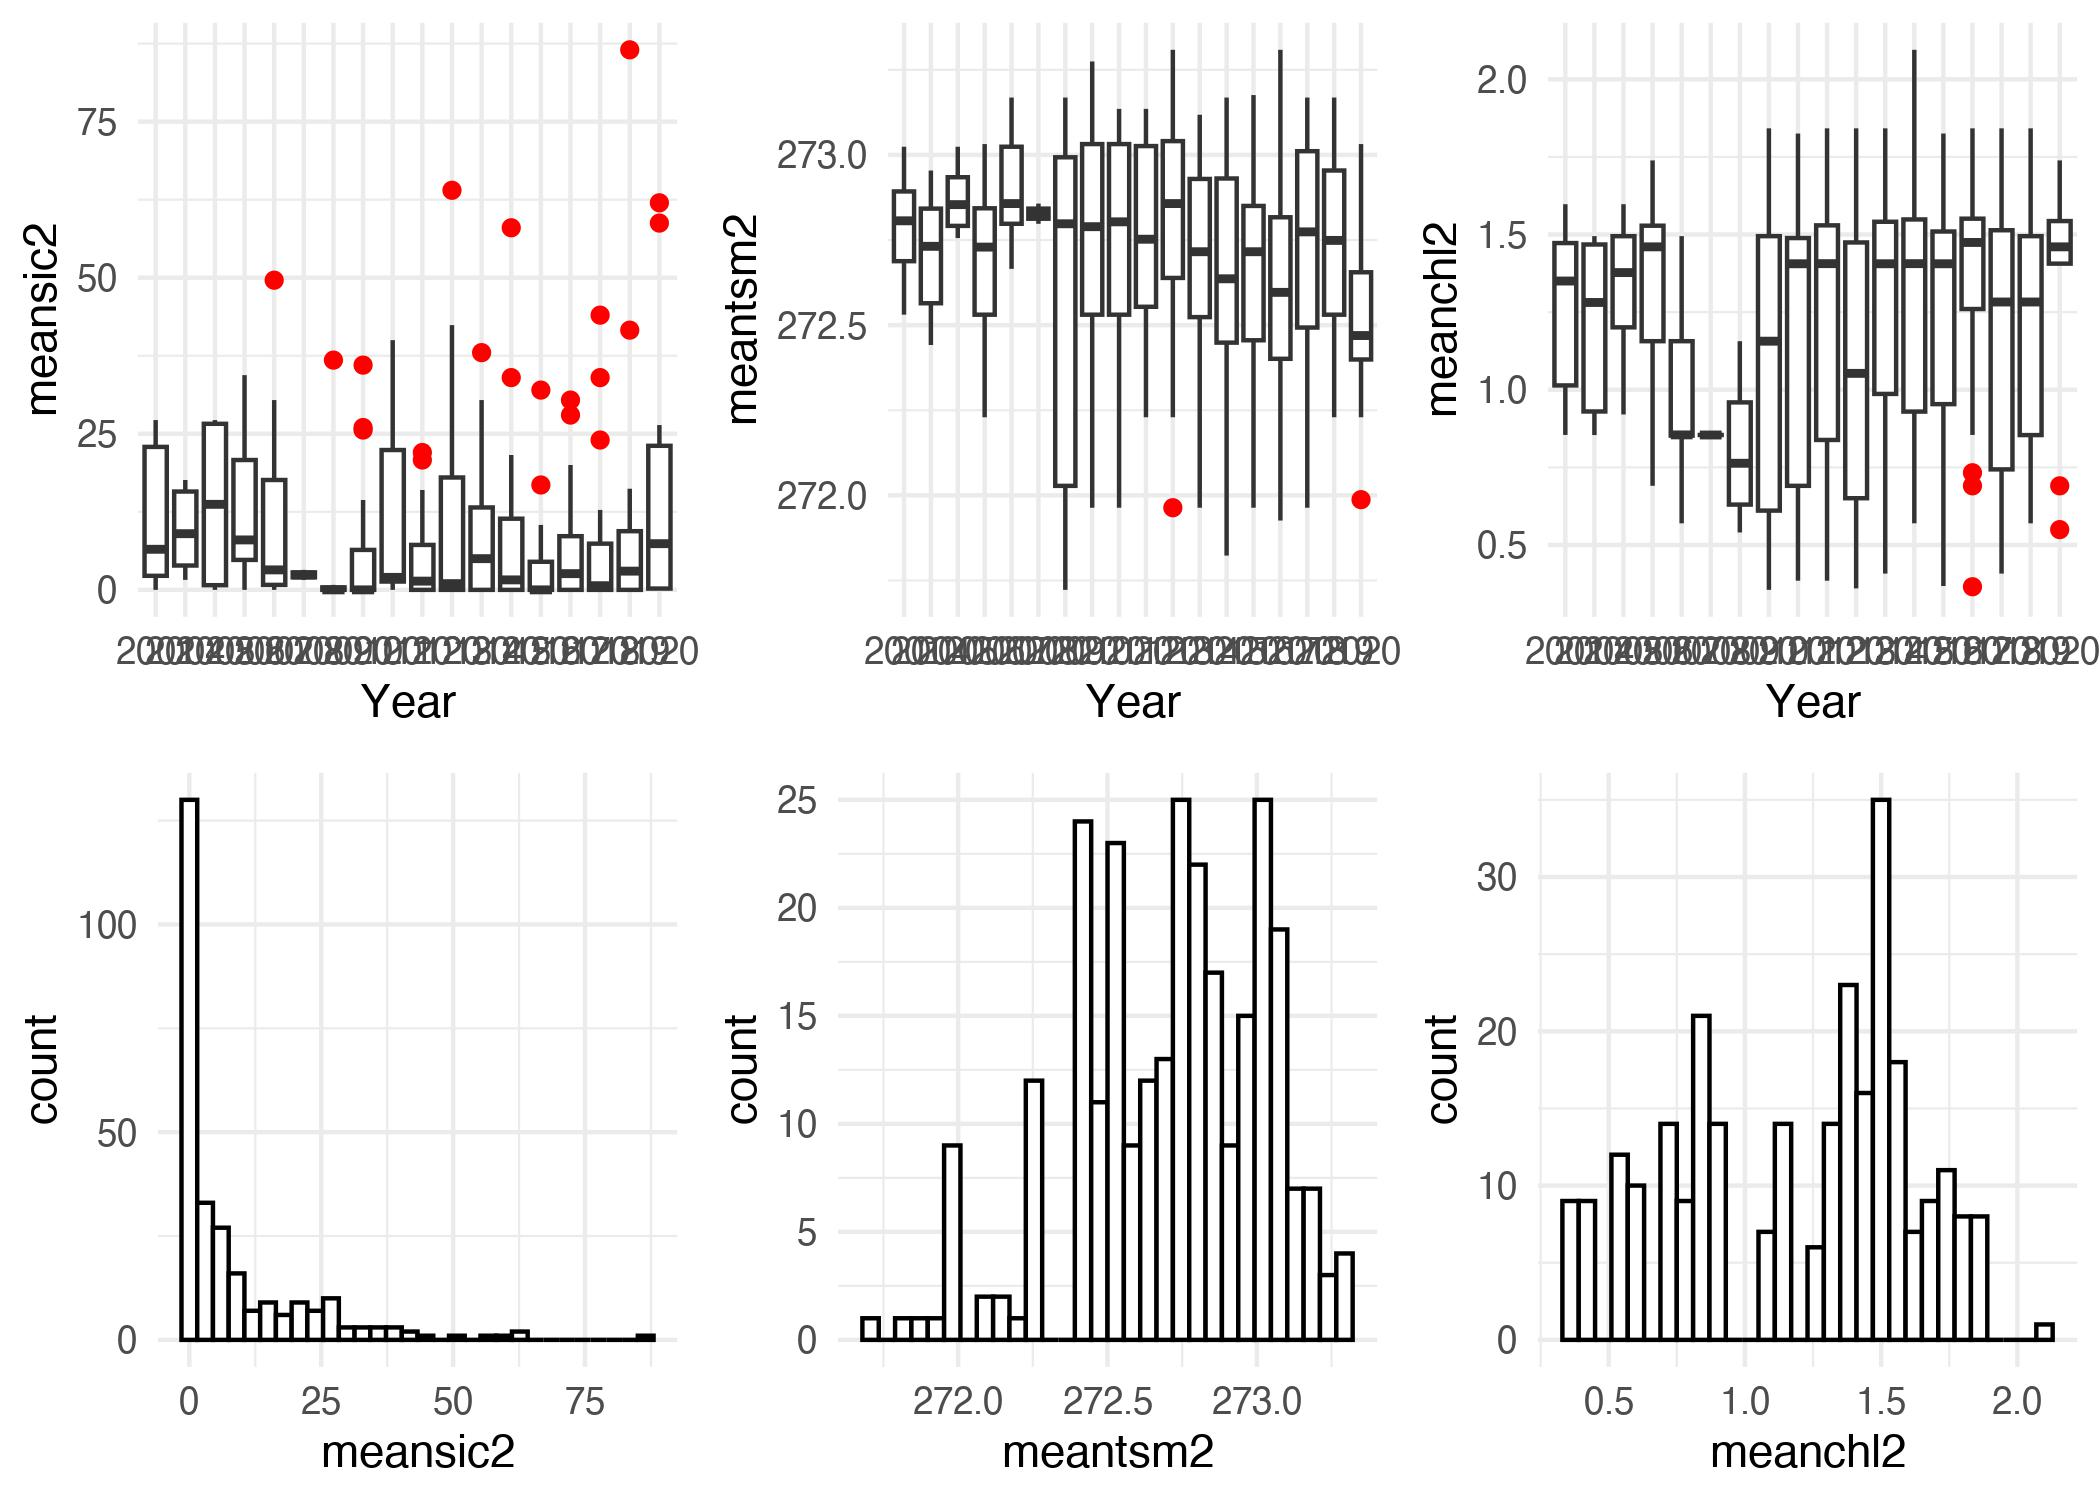
\includegraphics{indexPDF_files/figure-latex/unnamed-chunk-22-1} \end{center}

\newpage

\hypertarget{reading-length-strata-data}{%
\subsection{3.3. Reading length strata
data}\label{reading-length-strata-data}}

Brainsflied Strata

\begin{Shaded}
\begin{Highlighting}[]
\NormalTok{Lenbs }\OtherTok{\textless{}{-}} \FunctionTok{new}\NormalTok{(}\StringTok{"LB\_lengths"}\NormalTok{, }\AttributeTok{LB\_pars=}\NormalTok{MyPars, }\AttributeTok{file=}\FunctionTok{paste0}\NormalTok{(datdir, }\StringTok{"/Length\_481\_Krill\_2.csv"}\NormalTok{), }\AttributeTok{dataType=}\StringTok{"freq"}\NormalTok{,}\AttributeTok{sep=}\StringTok{";"}\NormalTok{,}\AttributeTok{header=}\NormalTok{T)}
\end{Highlighting}
\end{Shaded}

Elephan Island Strata

\begin{Shaded}
\begin{Highlighting}[]
\NormalTok{Lenei }\OtherTok{\textless{}{-}} \FunctionTok{new}\NormalTok{(}\StringTok{"LB\_lengths"}\NormalTok{, }\AttributeTok{LB\_pars=}\NormalTok{MyPars, }\AttributeTok{file=}\FunctionTok{paste0}\NormalTok{(datdir, }\StringTok{"/lenghtEI.csv"}\NormalTok{), }\AttributeTok{dataType=}\StringTok{"freq"}\NormalTok{,}\AttributeTok{sep=}\StringTok{";"}\NormalTok{,}\AttributeTok{header=}\NormalTok{T)}
\end{Highlighting}
\end{Shaded}

Extra Strata

\begin{Shaded}
\begin{Highlighting}[]
\NormalTok{Lenex }\OtherTok{\textless{}{-}} \FunctionTok{new}\NormalTok{(}\StringTok{"LB\_lengths"}\NormalTok{, }\AttributeTok{LB\_pars=}\NormalTok{MyPars, }\AttributeTok{file=}\FunctionTok{paste0}\NormalTok{(datdir, }\StringTok{"/lenghtExtra.csv"}\NormalTok{), }\AttributeTok{dataType=}\StringTok{"freq"}\NormalTok{,}\AttributeTok{sep=}\StringTok{";"}\NormalTok{,}\AttributeTok{header=}\NormalTok{T)}
\end{Highlighting}
\end{Shaded}

Join Strata

\begin{Shaded}
\begin{Highlighting}[]
\NormalTok{Lenjo }\OtherTok{\textless{}{-}} \FunctionTok{new}\NormalTok{(}\StringTok{"LB\_lengths"}\NormalTok{, }\AttributeTok{LB\_pars=}\NormalTok{MyPars, }\AttributeTok{file=}\FunctionTok{paste0}\NormalTok{(datdir, }\StringTok{"/lenghtJOIN.csv"}\NormalTok{), }\AttributeTok{dataType=}\StringTok{"freq"}\NormalTok{,}\AttributeTok{sep=}\StringTok{";"}\NormalTok{,}\AttributeTok{header=}\NormalTok{T)}
\end{Highlighting}
\end{Shaded}

SSIW Strata

\begin{Shaded}
\begin{Highlighting}[]
\NormalTok{Lenssiw }\OtherTok{\textless{}{-}} \FunctionTok{new}\NormalTok{(}\StringTok{"LB\_lengths"}\NormalTok{, }\AttributeTok{LB\_pars=}\NormalTok{MyPars, }\AttributeTok{file=}\FunctionTok{paste0}\NormalTok{(datdir, }\StringTok{"/lenghtSSIW.csv"}\NormalTok{), }\AttributeTok{dataType=}\StringTok{"freq"}\NormalTok{,}\AttributeTok{sep=}\StringTok{";"}\NormalTok{,}\AttributeTok{header=}\NormalTok{T)}
\end{Highlighting}
\end{Shaded}

\hypertarget{fit-the-model-by-strata}{%
\subsection{3.4. Fit the Model by
strata}\label{fit-the-model-by-strata}}

The LBSPR model is fitted using the \texttt{LBSPRfit} function:

\begin{Shaded}
\begin{Highlighting}[]
\NormalTok{fitbs }\OtherTok{\textless{}{-}} \FunctionTok{LBSPRfit}\NormalTok{(MyPars, Lenbs)}
\NormalTok{fitei }\OtherTok{\textless{}{-}} \FunctionTok{LBSPRfit}\NormalTok{(MyPars, Lenei)}
\NormalTok{fitex }\OtherTok{\textless{}{-}} \FunctionTok{LBSPRfit}\NormalTok{(MyPars, Lenex)}
\NormalTok{fitjo }\OtherTok{\textless{}{-}} \FunctionTok{LBSPRfit}\NormalTok{(MyPars, Lenjo)}
\NormalTok{fitssiw }\OtherTok{\textless{}{-}} \FunctionTok{LBSPRfit}\NormalTok{(MyPars, Lenssiw)}
\end{Highlighting}
\end{Shaded}

The smoother parameter estimates can be accessed from the \texttt{myFit}
object (which is an object of class LB\_obj {[}see earlier section for
details{]}): In this cae, we can look up estimates in Brainsfield Strata

\begin{Shaded}
\begin{Highlighting}[]
\NormalTok{fitei}\SpecialCharTok{@}\NormalTok{Ests}
\end{Highlighting}
\end{Shaded}

\begin{verbatim}
##        SL50  SL95   FM  SPR
##  [1,] 43.66 54.32 8.51 0.22
##  [2,] 43.10 53.47 8.17 0.21
##  [3,] 42.49 52.94 7.94 0.21
##  [4,] 42.48 52.71 7.80 0.22
##  [5,] 43.99 54.13 8.06 0.25
##  [6,] 44.51 54.19 8.01 0.27
##  [7,] 44.83 54.27 8.51 0.28
##  [8,] 45.12 54.14 8.76 0.29
##  [9,] 45.88 54.69 9.32 0.31
## [10,] 47.24 56.25 9.98 0.36
## [11,] 47.81 57.04 9.49 0.39
## [12,] 47.77 56.79 8.75 0.44
## [13,] 48.58 57.86 8.88 0.43
## [14,] 49.11 58.44 9.02 0.43
\end{verbatim}

Plotting fits by strata

Fit Bransfield

\begin{center}\includegraphics{indexPDF_files/figure-latex/unnamed-chunk-30-1} \end{center}

Fit Elephan Island

\begin{center}\includegraphics{indexPDF_files/figure-latex/unnamed-chunk-31-1} \end{center}

Fit Extra

\begin{center}\includegraphics{indexPDF_files/figure-latex/unnamed-chunk-32-1} \end{center}

Fit Join

\begin{center}\includegraphics{indexPDF_files/figure-latex/unnamed-chunk-33-1} \end{center}

Fit SSIW

\begin{center}\includegraphics{indexPDF_files/figure-latex/unnamed-chunk-34-1} \end{center}

Now we use \texttt{plotMat} function to know specified
maturity-at-length curve by strata, and the estimated
selectivity-at-length curve.

\begin{center}\includegraphics{indexPDF_files/figure-latex/unnamed-chunk-35-1} \end{center}

\begin{center}\includegraphics{indexPDF_files/figure-latex/unnamed-chunk-36-1} \end{center}

\begin{center}\includegraphics{indexPDF_files/figure-latex/unnamed-chunk-37-1} \end{center}

\begin{center}\includegraphics{indexPDF_files/figure-latex/unnamed-chunk-38-1} \end{center}

\begin{center}\includegraphics{indexPDF_files/figure-latex/unnamed-chunk-39-1} \end{center}

\hypertarget{comparing-producivity-between-strata}{%
\subsection{3.5. Comparing producivity between
Strata}\label{comparing-producivity-between-strata}}

For this, we extract \texttt{SPR} from each slot in the fits models by
strata.

Plot with all intrinsic productivity.

\begin{center}\includegraphics{indexPDF_files/figure-latex/unnamed-chunk-41-1} \end{center}

\newpage

\hypertarget{discussion}{%
\section{4. DISCUSSION}\label{discussion}}

(En la discusión se resumen, interpretan y extrapolan los resultados, se
analizan sus implicaciones y limitaciones, y se confrontan con las
hipótesis planteadas, considerando cómo ha sido la perspectiva de otros
autores.)

Identificar los cambios espaciales y temporales del krill en la PA ha
sido uno de los mayores desafíos durante los ultimos años. El krill es
una especie clave en el ambiente antartico y entender la dinamica
población es un elemento basico para visivilizar los impactos en el
funcionamenito de la trama trofica, conservacion del recurso y manejo de
la pesquería. nunestro interes fue dimiensionar el potencial
reproductivo de la especie a escalas finas de espacio y tiempo en la
subarea 48.1, dado que en esta area es donde se ha concentrado la
pesquería y el recurso durante los ultimos 20 años. Nuestro resultados
indentifican variabilidad espaciotemporal del krill en diferentes
estratos de manejo pesquero y a su vez fu posible proponer Pubtos
Biologicos de rewferencia en función de las caracteristicas de la
especie, lo cual constituye a su vez una recomendación para las actuales
estrategia de explotacion que lleva a cabo la CCMLAR. En este sentido,
identifican los periodos historicos pesqueros ren funcion del potencial
reproductivo y a su vez se propone un manejo espacialente explicito en
fincion de estos resultados

\hypertarget{cambios-en-estructura-poblacional-del-krill}{%
\subsection{4.1. Cambios en estructura poblacional del
Krill}\label{cambios-en-estructura-poblacional-del-krill}}

Las cambios en la dinámica y estructura poblacional en el krill en la
Península Antártica se manifiestan de varias maneras, como por ejemplo,
en la distribución, biomasa, , reclutamiento, fenología entre otras. Los
principales forzantes de estos cambios estan asociados al comportamiento
cambiante de las distintas variables ambientales en el habitat del krill
(\protect\hyperlink{ref-Saba2014}{Saba et al., 2014};
\protect\hyperlink{ref-Flores2012a}{\textbf{Flores2012a?}};
\protect\hyperlink{ref-Pinones2016}{\textbf{Pinones2016?}};
\protect\hyperlink{ref-Veytia2021}{\textbf{Veytia2021?}};
\protect\hyperlink{ref-Flores2012}{\textbf{Flores2012?}};
\protect\hyperlink{ref-Walsh2020}{\textbf{Walsh2020?}}). Frente a este
escenario cambiante, la productividad intrínseca poblacional, es decir,
el potencial reproductivo de la especie también ha sufrido cambios en
las ultimas decadas (\protect\hyperlink{ref-Atkinson2022}{Angus Atkinson
et al., 2022}; \protect\hyperlink{ref-Perry2020}{Perry, 2020};
\protect\hyperlink{ref-McBride2021}{\textbf{McBride2021?}}), tanto en la
escala temporal así como la espacial. De igual manera la estructura
poblacional del krill en la PA se ha visto impactada por este tipo de
forzantes ambientales (\protect\hyperlink{ref-Reiss2020}{Reiss et al.,
2020}; \protect\hyperlink{ref-Siegel2013}{Siegel et al., 2013})

equilibrium condition

\hypertarget{datos-pesqueros-como-indicadores-poblacionales}{%
\subsection{4.2. Datos pesqueros como indicadores
poblacionales}\label{datos-pesqueros-como-indicadores-poblacionales}}

El krill en la PA ha sido extraído comercialmente desde aproximadamente
1970 y constituye la pesquería mas grande del Océano Austral. Los datos
de la actividad pesquera en torno al krill han sido sistematicamente
colectados a bordo de las embarcaciones pesqueras a traves del programa
SISO, con lo cual ha sido posible tambien identificar cambios de la
dinamica poblacional que han ocurrido durantes las ultimas decada y
entoda la zona de mayor explotacion. Cambios en la disponibilidad,
distribucion, y concentracion, rendimiento del recurso se han visto
reflejados en los datos (\protect\hyperlink{ref-Kruger2019}{Krüger,
2019}; \protect\hyperlink{ref-SantaCruz2018}{Santa Cruz et al., 2018},
\protect\hyperlink{ref-SantaCruz2022}{2022};
\protect\hyperlink{ref-Atkinson2019a}{\textbf{Atkinson2019a?}}). Para
identificar cambios la productividad intrinseca de la población del
krill, utilizamos una de las piezas de información mas representativos
de la dinamica poblaciional de los recursos marinos explotados que
existen en este tipo de programas de monitoreo de pesquerías, en este
caso, datos de frecuencia de talla de la captura. {[}Hordyk et al.,
2014; Froese et al., 2018; Prince et al., 2015; Rudd y Thorson, 2018;
Ault et al., 2019; Chong et al., 2019; Pilling et al., 2008; Hordyk et
al., 2015; Mildenberger et al., 2017{]}. ; Froese et al., 2018). Este
tipo de datos son abundantes y permite cubrir una gran escala temporal y
espacial, en este caso, desde 1980 a 2020 y en toda la subarea 48.1
(Figura 1).

\hypertarget{diferencias-temporales-en-la-productividad-intrinseca-del-krill}{%
\subsection{4.3. Diferencias temporales en la productividad intrinseca
del
krill}\label{diferencias-temporales-en-la-productividad-intrinseca-del-krill}}

En terminos temporales, los estratos tienen diferencias en el potencial
reproductivo y por consiguiente en la productividad intrinseca de la
población. Durante los ultimos 20 años, el strato de elephant Island ha
tenido un aumento del potencial reporductivo lllegando a niveles del
56\% para el año 2020. Esto tiene relación con los cambios en los
niveles de produccón primaria que han suceido en esta zona. (cita)

Para demostrar esto, analizamos mas de 20 años de indicadores
poblacionales directos desde los datos de la pesquería para identificar
cambios de la productividad intrínseca en escalas espaciotemporales del
krill en la PA. Estos cambios fueron medidos cuantitativamente a través
del potencial reproductivo mediante un nobel método de uso común en
pesquerías del mundo que considera el uso de parametros de historia de
vida, como madurez, crecimiento y tasa de crecimiento, estructuras de
tallas y simulaciones basadas en paramettros invariantes

Cambios en la estructuración espacial de la población de krill han sido
demostradas de variadas maneras. A. Atkinson et al.
(\protect\hyperlink{ref-Atkinson2009}{2009}); A. Atkinson et al.
(\protect\hyperlink{ref-Atkinson2008}{2008}) indica que la población
muestra evidentes siítomas de contracción hacia el suroeste de la PA.
Esta contracción de la distribución de la población tiene consecuencias
otros fenomenos como en los rendimientos productivos que se manfiestan
en indicadores pesqueros como lo demuestra Santa Cruz et al.
(\protect\hyperlink{ref-SantaCruz2022}{2022}); Santa Cruz et al.
(\protect\hyperlink{ref-SantaCruz2018}{2018}).

\hypertarget{diferencias-espaciales-en-la-productividad-intrinseca-del-krill}{%
\subsection{4.4. Diferencias espaciales en la productividad intrinseca
del
krill}\label{diferencias-espaciales-en-la-productividad-intrinseca-del-krill}}

En este método determinamos las diferencias entre estructururas de
tallas simuladas del krill en función de sus parámetros de hisoria de
vida (Maschette et al. (\protect\hyperlink{ref-Maschette2020}{2020})) y
las resultantes de la pesquería, lo cua lpermite conocer la diferencia
entre el potencial reproductivo virginal y el que actualmente se
captura.

\hypertarget{comparacion-con-otros-estudios}{%
\subsection{4.5. Comparacion con otros
estudios}\label{comparacion-con-otros-estudios}}

Mace \& Sissenwine (1993) Review and meta-analysis of SPR reference
points for teleosts: 20\% SPR as limit reference points, \& 35-40\% SPR
for MSY that have been internationally recognized in the US, USA,
Australia, NZ etc. (\protect\hyperlink{ref-Goodyear1993}{Goodyear,
1993}; \protect\hyperlink{ref-Mace2001}{Mace, 2001}).

and increasing the mean length of krill, suggesting that recruitment
events are declining (\protect\hyperlink{ref-Atkinson2009}{A. Atkinson
et al., 2009})

cambios en el potencial reproductivo por zona:

Angus Atkinson et al. (\protect\hyperlink{ref-Atkinson2022}{2022}),
Perry (\protect\hyperlink{ref-Perry2020}{2020})

and have been used for assessments in the US South Atlantic, Pacific
islands, and Caribbean (Ehrhardt and Ault 1992; Ault et al.~2005, 2008;
Gedamke and Hoenig 2006; Nadon et al.~2015).

\hypertarget{consideraciones-finales}{%
\subsection{4.6. Consideraciones
finales}\label{consideraciones-finales}}

\begin{itemize}
\item
  Preliminar outputs to know intrinsic productivity of Antarctic krill
  (\emph{Euphausia superba}) in Antarctic Peninsula, SubArea 48.1.
\item
  This method dont incorportate environmental variables
\item
  Based in own krill dynamics
\item
  Do sensitivity analysis based on Linf (5 scenarios)
\item
  This code with methodology in this
  \href{https://github.com/MauroMardones/LBSPR_Krill}{link}
\end{itemize}

\newpage

\hypertarget{references}{%
\section*{5. REFERENCES}\label{references}}
\addcontentsline{toc}{section}{5. REFERENCES}

\hypertarget{refs}{}
\begin{CSLReferences}{1}{0}
\leavevmode\vadjust pre{\hypertarget{ref-Atkinson2022}{}}%
Atkinson, Angus, Hill, S. L., Reiss, C. S., Pakhomov, E. A., Beaugrand,
G., Tarling, G. A., Yang, G., Steinberg, D. K., Schmidt, K., Edwards,
M., Rombolá, E., \& Perry, F. A. (2022). {Stepping stones towards
Antarctica: Switch to southern spawning grounds explains an abrupt range
shift in krill}. \emph{Global Change Biology}, \emph{28}(4), 1359--1375.
\url{https://doi.org/10.1111/gcb.16009}

\leavevmode\vadjust pre{\hypertarget{ref-Atkinson2009}{}}%
Atkinson, A., Siegel, V., Pakhomov, E. A., Jessopp, M. J., \& Loeb, V.
(2009). {A re-appraisal of the total biomass and annual production of
Antarctic krill}. \emph{Deep-Sea Research Part I: Oceanographic Research
Papers}, \emph{56}(5), 727--740.
\url{https://doi.org/10.1016/j.dsr.2008.12.007}

\leavevmode\vadjust pre{\hypertarget{ref-Atkinson2008}{}}%
Atkinson, A., Siegel, V., Pakhomov, E. A., Rothery, P., Loeb, V., Ross,
R. M., Quetin, L. B., Schmidt, K., Fretwell, P., Murphy, E. J., Tarling,
G. A., \& Fleming, A. H. (2008). {Oceanic circumpolar habitats of
Antarctic krill}. \emph{Marine Ecology Progress Series},
\emph{362}(June), 1--23. \url{https://doi.org/10.3354/meps07498}

\leavevmode\vadjust pre{\hypertarget{ref-Beverton1957}{}}%
Beverton, R., \& Holt, S. (1957). \emph{{On the Dynamics of Exploited
Fish Populations}} (p. 540). SPRINGER-SCIENCE+BUSINES S MEDIA , B.V.

\leavevmode\vadjust pre{\hypertarget{ref-Canales2021}{}}%
Canales, C. M., Punt, A. E., \& Mardones, M. (2021). {Can a length-based
pseudo-cohort analysis (LBPA) using multiple catch length-frequencies
provide insight into population status in data-poor situations?}
\emph{Fisheries Research}, \emph{234}(October 2020), 105810.
\url{https://doi.org/10.1016/j.fishres.2020.105810}

\leavevmode\vadjust pre{\hypertarget{ref-Froese2018}{}}%
Froese, R., Winker, H., Coro, G., Demirel, N., Tsikliras, A. C.,
Dimarchopoulou, D., Scarcella, G., Probst, W. N., Dureuil, M., \& Pauly,
D. (2018). {A new approach for estimating stock status from length
frequency data}. \emph{ICES Journal of Marine Science}, \emph{76}(1),
350--351. \url{https://doi.org/10.1093/icesjms/fsy139}

\leavevmode\vadjust pre{\hypertarget{ref-Goodyear1993}{}}%
Goodyear, C. P. (1993). {Spawning stock biomass per recruit in fisheries
management: foundation and current use. }. \emph{Risk Evaluation and
Biological Reference Points for Fisheries Management}, \emph{120},
67--81.

\leavevmode\vadjust pre{\hypertarget{ref-LBSPR2021}{}}%
Hordyk, A. (2021). \emph{LBSPR: Length-based spawning potential ratio}.
\url{https://CRAN.R-project.org/package=LBSPR}

\leavevmode\vadjust pre{\hypertarget{ref-Hordyk2016}{}}%
Hordyk, A. R., Ono, K., Prince, J. D., \& Walters, C. J. (2016). {A
simple length-structured model based on life history ratios and
incorporating size-dependent selectivity: application to spawning
potential ratios for data-poor stocks}. \emph{Canadian Journal of
Fisheries and Aquatic Sciences}, \emph{73}(12), 1787--1799.
\url{https://doi.org/10.1139/cjfas-2015-0422}

\leavevmode\vadjust pre{\hypertarget{ref-Hordyk2014c}{}}%
Hordyk, A., Ono, K., Sainsbury, K., Loneragan, N., \& Prince, J. (2014).
\emph{{Spawning Potential Ratio}}. \emph{72}(2015), 204--216.

\leavevmode\vadjust pre{\hypertarget{ref-Jensen1996}{}}%
Jensen, A. L. (1996). {Beverton and Holt life history invariants result
from optimal trade-off of reproduction and survival}. \emph{Canadian
Journal of Fisheries and Aquatic Sciences}, \emph{53}(4), 820--822.
\url{https://doi.org/10.1139/f95-233}

\leavevmode\vadjust pre{\hypertarget{ref-Kruger2019}{}}%
Krüger, L. (2019). {Spatio-temporal trends of the Krill fisheries in the
Western Antarctic Peninsula and Southern Scotia Arc}. \emph{Fisheries
Management and Ecology}, \emph{26}(4), 327--333.
\url{https://doi.org/10.1111/fme.12363}

\leavevmode\vadjust pre{\hypertarget{ref-Mace2001}{}}%
Mace, P. M. (2001). {A new role for MSY in single-species and
ecosystem\(\backslash\)rapproaches to fisheries stock assessment and
management}. \emph{Fish and Fisheries}, \emph{2}, 2--32.
\url{https://doi.org/10.1046/j.1467-2979.2001.00033.x}

\leavevmode\vadjust pre{\hypertarget{ref-Maschette2020}{}}%
Maschette, D., Wotherspoon, S., Pavez, C., Ziegler, P., Thanassekos, S.,
Reid, K., Kawaguchi, S., Welsford, D., \& Constable, A. (2020).
\emph{{Generalised R Yield Model (Grym)}}.
\url{https://www.ccamlr.org/en/system/files/meeting\%7B/_\%7Ddocuments/with\%7B/_\%7Dcover/sc-39-bg-19.pdf}

\leavevmode\vadjust pre{\hypertarget{ref-Perry2020}{}}%
Perry, F. (2020). \emph{{Antarctic krill recruitment in the south-west
Atlantic sector of the Southern Ocean}} (p. 310) {[}PhD thesis{]}.
UNIVERSITY OF SOUTHAMPTON.

\leavevmode\vadjust pre{\hypertarget{ref-Prince2018}{}}%
Prince, J., \& Hordyk, A. (2018). \emph{{What to do when you have almost
nothing : A simple quantitative prescription for managing extremely
data- ­ poor fisheries}}. \emph{May}, 1--15.
\url{https://doi.org/10.1111/faf.12335}

\leavevmode\vadjust pre{\hypertarget{ref-Reiss2020}{}}%
Reiss, C. S., Hinke, J. T., \& Watters, G. M. (2020). {Demographic and
maturity patterns of Antarctic krill (Euphausia superba) in an
overwintering hotspot}. \emph{Polar Biology}, \emph{43}(9), 1233--1245.
\url{https://doi.org/10.1007/s00300-020-02704-4}

\leavevmode\vadjust pre{\hypertarget{ref-Rudd2017a}{}}%
Rudd, M. B., \& Thorson, J. T. (2017). {Accounting for variable
recruitment and fishing mortality in length-based stock assessments for
data-limited fisheries}. \emph{Canadian Journal of Fisheries and Aquatic
Sciences}, \emph{75}(7), 1019--1035.
\url{https://doi.org/10.1139/cjfas-2017-0143}

\leavevmode\vadjust pre{\hypertarget{ref-Saba2014}{}}%
Saba, G. K., Fraser, W. R., Saba, V. S., Iannuzzi, R. A., Coleman, K.
E., Doney, S. C., Ducklow, H. W., Martinson, D. G., Miles, T. N.,
Patterson-Fraser, D. L., Stammerjohn, S. E., Steinberg, D. K., \&
Schofield, O. M. (2014). {Winter and spring controls on the summer food
web of the coastal West Antarctic Peninsula}. \emph{Nature
Communications}, \emph{5}. \url{https://doi.org/10.1038/ncomms5318}

\leavevmode\vadjust pre{\hypertarget{ref-SantaCruz2018}{}}%
Santa Cruz, F., Ernst, B., Arata, J. A., \& Parada, C. (2018). {Spatial
and temporal dynamics of the Antarctic krill fishery in fishing hotspots
in the Bransfield Strait and South Shetland Islands}. \emph{Fisheries
Research}, \emph{208}(August), 157--166.
\url{https://doi.org/10.1016/j.fishres.2018.07.020}

\leavevmode\vadjust pre{\hypertarget{ref-SantaCruz2022}{}}%
Santa Cruz, F., Krüger, L., \& Cárdenas, C. A. (2022). {Spatial and
temporal catch concentrations for Antarctic krill: Implications for
fishing performance and precautionary management in the Southern Ocean}.
\emph{Ocean {\&} Coastal Management}, \emph{223}(September 2021),
106146. \url{https://doi.org/10.1016/j.ocecoaman.2022.106146}

\leavevmode\vadjust pre{\hypertarget{ref-Siegel2013}{}}%
Siegel, V., Reiss, C. S., Dietrich, K. S., Haraldsson, M., \& Rohardt,
G. (2013). {Distribution and abundance of Antarctic krill (Euphausia
superba) along the Antarctic Peninsula}. \emph{Deep-Sea Research Part I:
Oceanographic Research Papers}, \emph{77}, 63--74.
\url{https://doi.org/10.1016/j.dsr.2013.02.005}

\leavevmode\vadjust pre{\hypertarget{ref-Stammerjohn2008a}{}}%
Stammerjohn, Sharon E., Martinson, D. G., Smith, R. C., \& Iannuzzi, R.
A. (2008). {Sea ice in the western Antarctic Peninsula region:
Spatio-temporal variability from ecological and climate change
perspectives}. \emph{Deep-Sea Research Part II: Topical Studies in
Oceanography}, \emph{55}(18-19), 2041--2058.
\url{https://doi.org/10.1016/j.dsr2.2008.04.026}

\leavevmode\vadjust pre{\hypertarget{ref-Stammerjohn2008}{}}%
Stammerjohn, S. E., Martinson, D. G., Smith, R. C., Yuan, X., \& Rind,
D. (2008). {Trends in Antarctic annual sea ice retreat and advance and
their relation to El Ni{ñ}o-Southern Oscillation and Southern Annular
Mode variability}. \emph{Journal of Geophysical Research: Oceans},
\emph{113}(3), 1--20. \url{https://doi.org/10.1029/2007jc004269}

\leavevmode\vadjust pre{\hypertarget{ref-Thanassekos2014}{}}%
Thanassekos, S., Cox, M. J., \& Reid, K. (2014). {Investigating the
effect of recruitment variability on length-based recruitment indices
for antarctic krill using an individual-based population dynamics
model}. \emph{PLoS ONE}, \emph{9}(12), 1--20.
\url{https://doi.org/10.1371/journal.pone.0114378}

\leavevmode\vadjust pre{\hypertarget{ref-Dornam2021}{}}%
WG-EMM-2021/05. (2021). \emph{{Results from the WG-ASAM intersessional
e-group on Krill biomass estimates from acoustic surveys.
WG-EMM-2021/05. WG-ASAM e-group on Krill biomass estimates from acoustic
surveys.}} (p. 16). Commission for the Conservation of Antarctic Marine
Living Resources (CCAMLR).

\leavevmode\vadjust pre{\hypertarget{ref-Zhou2012}{}}%
Zhou, S., Yin, S., Thorson, J. T., Smith, A. D. M., Fuller, M., \&
Walters, C. J. (2012). {Linking fishing mortality reference points to
life history traits: an~empirical study}. \emph{Canadian Journal of
Fisheries and Aquatic Sciences}, \emph{69}(8), 1292--1301.
\url{https://doi.org/10.1139/f2012-060}

\end{CSLReferences}

\end{document}
